\section{Introducción}
En este capítulo, se usará el modelo de redes neuronales recurrentes con unidades LSTM para analizar la distribución de sucesiones cuyos valores sean reales. Por lo tanto, siguiendo el trabajo de (Graves, 2013), se utilizará la base de datos de caligrafía en línea de IAM (IAM-OnDB) \cite{handwriting}. 
Se llama caligrafía en línea porque la escritura está registrada como sucesiones de la ubicación de la punta de la pluma. Estos datos son atractivos para la generación de sucesiones debido a su baja dimensionalidad, dos números reales por cada punto, y su facilidad de visualización. 
\cite{handwriting}
\cite{DBLP:journals/corr/Graves13}


\vspace{1em}

Siguiendo a (Graves, 2013), el objetivo del capítulo será de generar caligrafía en línea con buena legibilidad. Por esta razón y porque no existen $``$benchmarks$"$ relevantes, los resultados de validación pasarán a segundo plano. Por otro lado, determinar una distribución predictiva que funcione bien con los datos de entrada fue el principal reto para Graves. El modelo que decidió utilizar el científico tiene tres componentes principales: las unidades de memoria LSTM, un mecanismo de atención y una mezcla de gaussianas como capa de salida para generar una red de densidad mixta. 

\vspace{1em}

En el siguiente capítulo, se comenzará por dar más detalles sobre la base de datos utilizada, después se explicará el modelo empleado y, finalmente, se mostrarán los resultados obtenidos.


\section{Descripción de la base de datos}
La base de datos IAM-OnDB consiste de enunciados de caligrafía en línea registrados a partir de 221 escritores diferentes utilizando un $``$pizarrón inteligente$"$. A los escritores se les pidió escribir enunciados contenidos en la base de texto Lancaster-Oslo-Bergen y la posición de su pluma fue registrada utilizando un dispositivo infrarojo en la esquina del pizarrón. Los datos originales contienen las coordenadas $(x,y)$ de los puntos además de otra variable que indica en qué puntos se levantó la pluma del pizarrón. Predecir el movimiento de la pluma un punto a la vez permite al modelo tener máxima flexibilidad para inventar caligrafía nueva, pero también requiere mucha memoria. La letra promedio ocupa más de 25 periodos y el enunciado promedio alrededor de 700. En la figura 5.1, tomada de (Graves, 2013) se puede ver una muestra de los datos
\cite{DBLP:journals/corr/Graves13}

\begin{figure}[h]
\begin{center}
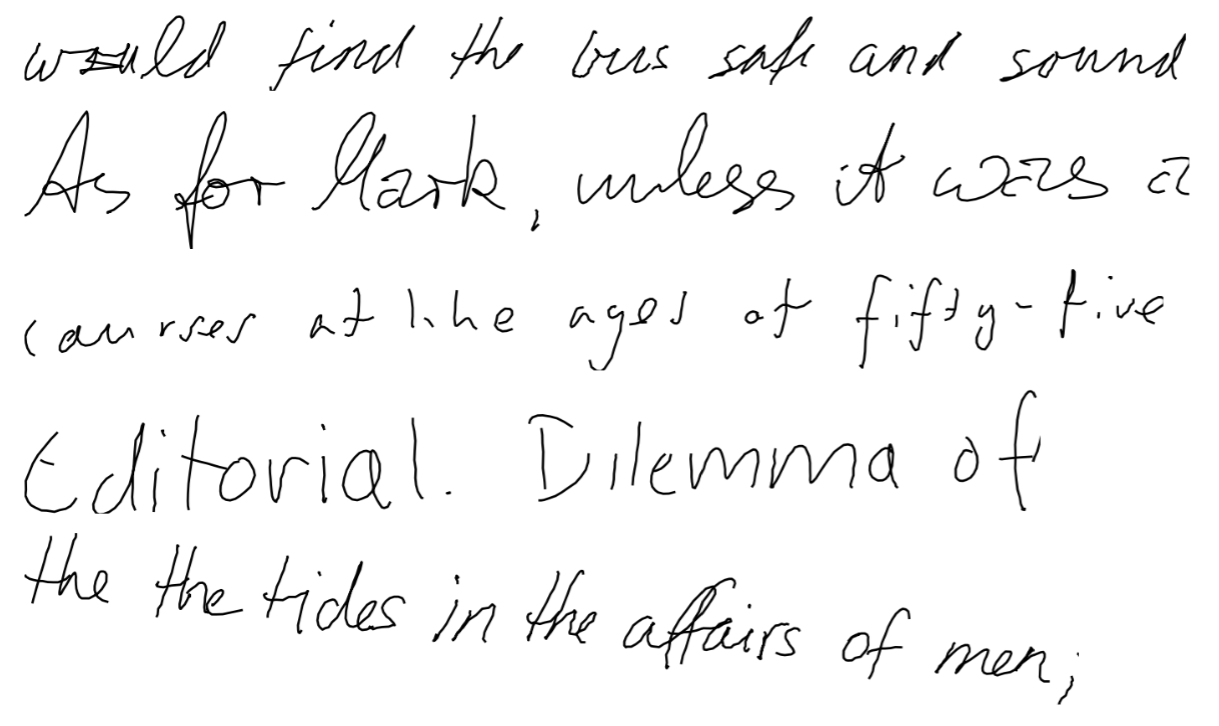
\includegraphics{./imag/iam.png}
\end{center}
\caption{}
\end{figure}

\section{Descripción del modelo}
Como se mencionó en la introducción del capítulo, el modelo utilizado para este experimento tiene 3 partes principales: las unidades de memoria LSTM, un mecanismo de atención y una red de densidad mixta. Las unidades de memoria LSTM se explicaron en el capítulo 3, por lo que, en esta sección, se explicará cómo funciona la densidad mixta en el modelo y después se describirá el mecanismo de atención. 

\subsection{Red de densidad mixta}
En la sección 3.2, se dio una breve introducción a redes de densidad mixtas. El objetivo de estas es usar los datos de salida de una red neuronal para parametrizar una mezcla de distribuciones. Una parte de los datos de salida se usan para definir los pesos de mezcla y el resto para parametrizar las componentes de las mezclas individuales. Los pesos de mezcla se normalizan con una función softmax y a los demás datos de salida se les aplican funciones adecuadas para mantener sus valores en un rango adecuado. La red de densidad mixta se entrena maximizando la log probabilidad de los objetivos bajo las distribuciones inducidas.
\cite{DBLP:journals/corr/Graves13}

\vspace{1em}

Cada vector de entrada $x_t$ consiste de un par de números reales $x_1,x_2$ que define la desviación de la pluma con respecto al dato de entrada anterior, y una variable binaria $x_3$ que tiene valor 1 cuando el vector termina un trazo, es decir, si la pluma fue levantada del pizarrón antes que el siguiente vector fuera registrado. Una mezcla de gaussianas bivariadas fue usada para predecir $x_1$ y $x_2$, mientras que una distribución Bernoulli fue usada para $x_3$. Cada vector de salida $y_t$ consiste de la probabilidad de fin de trazo $e$, un conjunto de medias $\mu^j$, desviaciones estandar $\sigma^j$, correlaciones $\rho^j$ y pesos de mezcla $\pi^j$ para las $M$ componentes de mezcla. A continuación se pueden ver las ecuaciones que se describieron siguiendo a (Graves, 2013).
\cite{DBLP:journals/corr/Graves13}

\begin{equation}
\begin{split}
$$x_t \in \mathbb{R} \times \mathbb{R} \times \{0,1\} $$
\end{split}
\end{equation}
\begin{equation}
\begin{split}
$$y_t = \left( e_t , \{\pi^j_t, \mu^j_t, \sigma^j_t, \rho^j_t \}_{j=1}^M \right) $$
\end{split}
\end{equation}

La media y desviación estandar son vectores de dimensión 2, mientras que el peso, la correlación y la probabilidad de término de trazo son escalares. Los vectores $y_t$ se obtienen de los datos de salida de la red $\hat{y_t}$ de la siguiente manera:
\cite{DBLP:journals/corr/Graves13}

\begin{equation}
\begin{split}
$$\hat{y_t} = \left( \hat{e_t} , \{\hat{w}_t^j, \hat{\mu}_t^j, \hat{\sigma}_t^j, \hat{\rho}_t^j \}_{j=1}^M  \right) = b_y + \sum_{n=1}^N W_{h^ny}h_t^n $$
\end{split}
\end{equation}
\begin{equation}
\begin{split}
$$e_t = \frac{1}{1+exp(\hat{e}_t)}$$
\end{split}
\end{equation}
\begin{equation}
\begin{split}
$$\pi_t^j = \frac{exp(\hat{\pi}_t^j)}{\sum_{j'=1}^M exp(\hat{\pi}_t^{j'}) }$$
\end{split}
\end{equation}
\begin{equation}
\begin{split}
$$\sigma_t^j = exp(\hat{\sigma}_t^j)$
\end{split}
\end{equation}

\begin{equation}
\begin{split}
$$\rho_t^j = tanh(\hat{\rho}_t^j)$$
\end{split}
\end{equation}

La función de densidad $Pr(x_{t+1}|y_t)$ para el siguiente dato de entrada $x_{t+1}$ dado el vector de salida $y_t$ se define de la siguiente manera:

\begin{equation}
\begin{split}
Pr(x_{t+1}|y_t)=\sum_{j=1}^{M} \pi_t^j  \mathcal{N}(x_{t+1}|\mu_t^j,\sigma_t^j,\rho_t^j)
\left\{
        \begin{array}{ll}
            e_t & (x_{t+1})_3=1\\
            1-e_t & \quad \mathrm{eoc}
        \end{array}
    \right.
\end{split}
\end{equation}

donde
\begin{equation}
\begin{split}
$$\mathcal{N}(x|\mu, \sigma, \rho)=\frac{1}{2\pi\sigma_1\sigma_2\sqrt{1 - \rho^2}} \mathrm{exp}\left[ \frac{-Z}{2(1-\rho^2)}\right]$$
\end{split}
\end{equation}

con
\begin{equation}
\begin{split}
$$Z = \frac{(x_1 - \mu_1)^2}{\sigma_1^2} + \frac{(x_2 - \mu_2)^2}{\sigma_2^2} - \frac{2\rho(x_1 - \mu_1)(x_2 - \mu_2)}{\sigma_1 \sigma_2}$$
\end{split}
\end{equation}
Por lo tanto, si se utiliza la función de pérdida logarítmica, al sustituir las ecuaciones (5.3.9) y (5.3.10), se obtendrá la siguiente función de pérdida

\begin{equation}
\begin{split}
\mathcal{L}(x)=\sum_{t=1}^{T} -log\left(\sum_{j} \pi_t^j\mathcal{N}(x_{t+1}|\mu_t^j,\sigma_t^j,\rho_t^j)
\right)
-\left\{
        \begin{array}{ll}
            \log e_t & (x_{t+1})_3=1\\
            \log(1-e_t) & \quad \mathrm{eoc}
        \end{array}
    \right.
\end{split}
\end{equation}

\vspace{1em}

En la figura 5.2, se puede ver la operación de la capa de densidad mixta aplicada a una predicción de caligrafía al escribir a palabra $``$itam$"$. Aquí se puede ver que hay dos tipos de predicción en el modelo: las pequeñas burbujas que denotan los trazos que se hacen al escribir las letras, y unas burbujas más grandes que son las predicciones al terminar un trazo y para comenzar el siguiente. Las predicciones al final de los trazos tienen una varianza más alta porque la posición de la pluma no fue registrada cuando estuvo despegada del pizarrón y, por lo tanto, puede haber una distancia más grande entre el final de un trazo y el siguiente.
\cite{DBLP:journals/corr/Graves13}

\begin{figure}[h]
\begin{center}
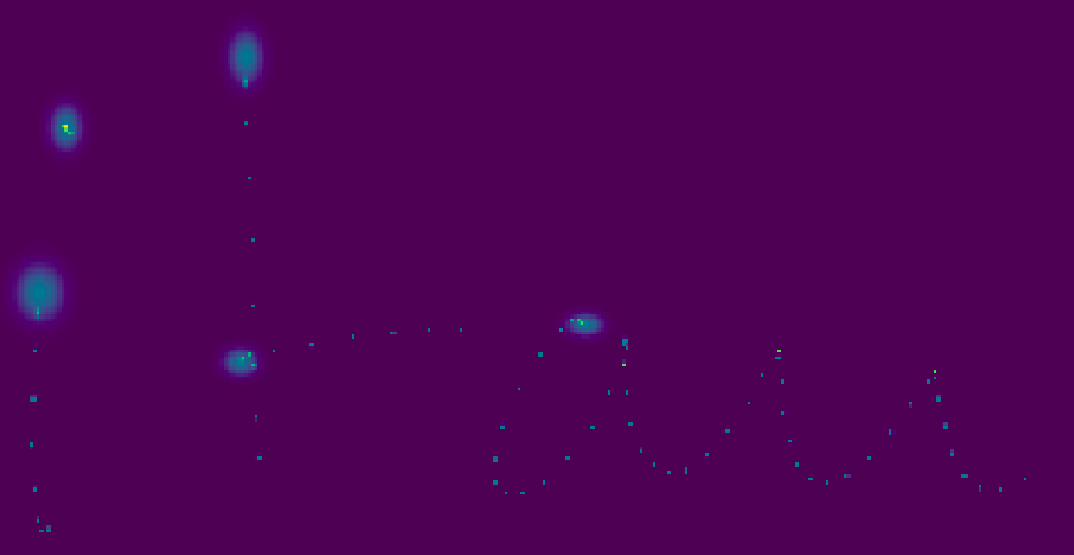
\includegraphics{./imag/mdn.png}
\end{center}
\caption{}
\end{figure}

\vspace{1em}

La capa de densidad mixta es muy útil para generar caligrafía convincente. Sin embargo, todavía hace falta la parte del modelo que permitirá generar las sucesiones de texto que se requieran. Esta parte del modelo, llamada mecanismo de atención, se presentará a continuación.

\subsection{Mecanismos de atención}
Para poder generar caligrafía para un cierto texto dado, se condicionarán las predicciones de la caligrafía en el texto que se quiere escribir. Sin embargo, uno de los problemas más importantes al tratar de hacer esto es que la sucesión de caligrafía es 25 veces más grande en promedio que el texto. Otro reto es que la alineación entre el texto y la caligrafía no se conoce hasta que los datos son generados debido a que el número de coordenadas usadas para escribir cada caracter cambia de manera importante de acuerdo al estilo, tamaño, velocidad de la pluma, etc. 
\cite{DBLP:journals/corr/Graves13}

\vspace{1em}

Para resolver este problema, siguiendo a (Graves, 2013), en este trabajo se creará una mecanismo de atención que consiste de una $``$ventana suave$"$ que es convolucionada con el texto y luego alimentada como dato de entrada para la red de predicción. Los parámetros de la ventana se obtienen del modelo al mismo tiempo que se hacen las predicciones, para que dinámicamente se determine una alineación entre la ubicación del texto y de la pluma. En otras palabras, el modelo aprende a decidir que caracter escribir después.

\vspace{1em}

La ventana suave se define a continuación. Dada una sucesión $c$ con $U$ caracteres, la ventana suave $w_t$ con respecto al paso de tiempo $t$ $(1 \leq t \leq T)$ se define mediante la siguiente convolución con una mezcla de $K$ funciones gaussianas donde $\phi(t,u)$ es el peso de la ventana de $c_u$ en el tiempo $t$.
\cite{DBLP:journals/corr/Graves13}

\begin{equation}
\begin{split}
$$\phi(t,u) = \sum_{k=1}^K \alpha_t^k \mathrm{exp}\left(-\beta_t^k(\kappa_t^k - u)^2\right)$$
\end{split}
\end{equation}
\begin{equation}
\begin{split}
$$w_t = \sum_{u=1}^U \phi(t,u)c_u$$
\end{split}
\end{equation}

Intuitivamente, explica Graves, el parámetro $\kappa_t$ controla la ubicación de la ventana, los parámetros $\beta_t$ controlan el ancho de la ventana y los parámetros $\alpha_t$ controlan la importancia de la ventana dentro de la mezcla. Por otro lado, los parámetros de la ventana se calculan de la siguiente manera a partir de los datos de salida de la primera capa oculta del modelo.
\cite{DBLP:journals/corr/Graves13}

\begin{equation}
\begin{split}
$$(\hat{\alpha}_t, \hat{\beta}_t, \hat{\kappa}_t) = W_{h^1p}h_t^1 +b_p$$
\end{split}
\end{equation}
\begin{equation}
\begin{split}
$$\alpha_t = \mathrm{exp}(\hat{\alpha})$$
\end{split}
\end{equation}
\begin{equation}
\begin{split}
$$\beta_t = \mathrm{exp}(\hat{\beta})$$
\end{split}
\end{equation}
\begin{equation}
\begin{split}
$$\kappa_t = \kappa_{t-1} + \mathrm{exp}(\hat{\kappa})$$
\end{split}
\end{equation}

Los parámetros de ubicación $\kappa_t$ se definen como la diferencia con respecto a la ubicación anterior $c_{t-1}$ para poder alinear el texto con el trazo de la pluma. Después de esto, los vectores $w_t$ se pasan hacia las siguientes capas ocultas en el tiempo $t$ y hacia la primera capa oculta en el tiempo $t+1$ como datos de entrada.


\section{Resultados}

A continuación se mostrarán los resultados que entregó el algoritmo implementado por el autor. El código se puede encontrar en http://github.com/GeorBelanger/

\vspace{1em}

Para elegir los hiperparámetros del modelo, se tomó como base (Graves, 2013). Sin embargo, debido a que no se contaba con la suficiente capacidad computacional, se redujeron algunos parámetros para poder entrenar el modelo en un tiempo razonable, como por ejemplo el número de unidades LSTM en cada capa oculta.

\vspace{1em}

El modelo utilizó 3 capas ocultas con 200 unidades LSTM en cada una, los batches con tamaño 64, 8 gaussianas en la capa de salida, a rmsprop como algoritmo de optimización y recorte de gradiente a 10. La red recurrente se desenrolló 150 pasos de tiempo y el promedio de pasos de tiempo o trazos de cada letra se fijo en 25. Por lo que el algoritmo se fija en promedio en las 6 letras anteriores para hacer el siguiente trazo. Para la generación de sucesiones, se escogieron frases que tuvieran que ver con la misión, filosofía o mercadotecnia del ITAM.

\vspace{1em}

 En la figura 5.3, se puede ver generación de caligrafía condicionada en la frase: $``$Por un México más libre$"$ después de la iteración 4700 del algoritmo. En esta primera prueba, solo se generaron los primeros 6 caracteres de las sucesiones, contando al espacio.


\begin{figure}[h]
\begin{center}
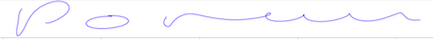
\includegraphics{./imag/porunmexico4700.png}
\end{center}
\caption{}
\end{figure}

Se puede ver que el algoritmo ya comienza a aprender a escribir las letras. En la figura 5.4, se puede ver la operación de la capa de densidad mixta aplicada a este ejemplo.

\begin{figure}[h]
\begin{center}
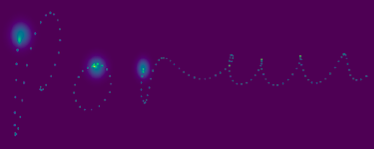
\includegraphics{./imag/porunmexico4700g.png}
\end{center}
\caption{}
\end{figure}

Se intentaron construir sucesiones más largas. En la figura 5.5, se puede ver la generación de caligrafía basada en la frase $``$solo hay un itam$"$ que se produjo en la iteración 7,500. Se puede ver que la primera parte de la frase la escribe sin problemas pero después de escribir "un", parece que pierde un poco el rumbo. La alineación entre el texto que se quiere escribir y la caligrafía, manejada por el mecanismo de atención, todavía tiene algunas fallas


\begin{figure}[h]
\begin{center}
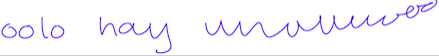
\includegraphics{./imag/solo7500.png}
\end{center}
\caption{}
\end{figure}

\vspace{1em}

En la figura 5.6, se puede ver la generación de caligrafía basada en la frase $``$contribuir a la formación integral $"$ que se produjo en la iteración 8,700. Se puede ver que ya escribe bastante bien y el mecanismo de atención funciona en general, aunque en algunos lugares falla, como en la doble $``$b$"$ que se ve en la figura 5.6. Esto se debe probablemente el mecanismo de atención estuvo demasiados pasos de tiempo $``$dibujando$"$ a $``$b$"$ y entonces la dibujó dos veces. 


\begin{figure}[h]
\begin{center}
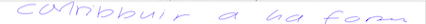
\includegraphics{./imag/contribuir8700.png}
\end{center}
\caption{}
\end{figure}

Para la iteración 10,000, el modelo ya ha aprendido a seguir las letras utilizando el mecanismo de atención, aunque todavía hay algunas letras que tienen algunos problemas. Por ejemplo, en la figura 5.7, se ve la escritura de $``$Por un México más libre$"$. Se puede ver que el error más grande fue que el algoritmo no produjo la $``$x$"$ de México. Esto se debe probablemente a que como la $``$x$"$ es una letra poco común, el mecanismo de atención no ha tenido suficientes ejemplos para aprender a hacerla.

\begin{figure}[htbp]
\begin{center}
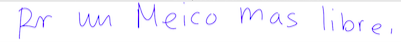
\includegraphics{./imag/por_un_10000.png}
\end{center}
\caption{}
\end{figure}

Para completar el lema del ITAM, en la figura 5.8, se puede ver la generación del texto $``$más justo y más próspero$"$. Aquí el algoritmo tiene problemas para escribir las $``$s$"$, y al final de $``$próspero$"$, todavía quedan trazos por hacer, por lo que aparece una $``$n$"$ $``$no invitada$"$ al final.

\begin{figure}[htbp]
\begin{center}
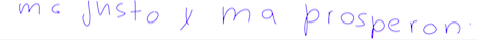
\includegraphics{./imag/justo10000.png}
\end{center}
\caption{}
\end{figure}

\vspace{3em}

Por último, en las figuras 5.9 y 5.10, se puede ver la generación del texto $``$solo hay un itam$"$. El algoritmo escribe bastante bien esta frase. Ha aprendido a escribir las letras y seguir de manera adecuada al mecanismo de atención.  La única falla que tuvo es que tal vez falta un poco de espacio entre la palabra $``$un$"$ y la palabra $``$itam$"$.

\begin{figure}[htbp]
\begin{center}
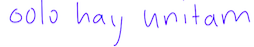
\includegraphics{./imag/solo4.png}
\end{center}
\caption{}
\end{figure}
\begin{figure}[htbp]
\begin{center}
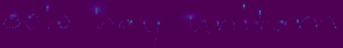
\includegraphics{./imag/solo5.png}
\end{center}
\caption{}
\end{figure}

\vspace{3em}

Los resultados aquí expuestos muestran el poder que tienen los modelos explicados para generar sucesiones complejas de dependencias de largo plazo. La calidad de la escritura todavía podría mejorar si como (Graves, 2013) se utilizara un modelo más grande y se entrenara por más tiempo. Sin embargo, no se cuenta con la capacidad computacional necesaria y para este trabajo bastará mostrar el potencial que tienen los modelos.
\cite{DBLP:journals/corr/Graves13}